\documentclass[22pt]{beamer}
\usepackage[orientation=portrait, size=custom, width=91.44, height=91.44,scale=1.2]{beamerposter} % 36in*2.5 = 90cm
\usepackage[absolute,overlay]{textpos}
\usepackage{bookmark} %pdflatex says to use this to avoid errors...
\usepackage{graphicx} %for including images
\graphicspath{{figs/}} %location of images
\usepackage{wrapfig} %wrap text around the images
\usepackage{listingsutf8}    %package for code environment; use this instead of verbatim to get automatic line break; use this instead of listings to get (•)
\usepackage{amsmath}
\usepackage{gensymb}
\usepackage[export]{adjustbox}
\usepackage[skins,theorems]{tcolorbox}
\usepackage{tikz}
\newcommand*\circled[1]{\tikz[baseline=(char.base)]{
            \node[shape=circle,draw,inner sep=2pt] (char) {#1};}}
\usepackage{array}
\usepackage{booktabs,adjustbox}
\usepackage{subcaption}
\usepackage{pgfplots}
%plot options
\pgfplotsset{width=7cm,compat=1.8}
\PassOptionsToPackage{gray}{xcolor}

\usetikzlibrary{shapes,shapes.geometric,arrows,fit,calc,positioning,automata,}

\usepackage{wrapfig}

%\mode<presentation>
%this doesn't seem to make any difference; leave for now for trying out
\usetheme{Berlin}
\definecolor{MacBlue}{rgb}{0.10196,0.22353,0.53725}
\definecolor{MacMaroon} {rgb}{0.47843, 0, 0.23137}
\definecolor{MacMaroon2} {rgb}{0.47451, 0, 0}
\definecolor{MacGray}{rgb}{0.50196,0.49804,0.51765}
\definecolor{MacMaroon3}{rgb}{00.47,0.2,0.31}
\definecolor{MacGold}{rgb}{1, 0.75,0.35}
\usecolortheme[named=MacMaroon2]{structure}
\setbeamertemplate{caption}[numbered]
\setbeamertemplate{navigation symbols}{}

\title{Adventures in 3D: \\Creating and Delivering Tools for 3D Remote Camps for Middle Schoolers}
\subtitle{}  %probably want a better subtitle
  \author[Yao, Lee, Wu, Wang, Schankula, \& Anand]
      {Larry Yao, Jiwoo Lee, Sharon Wu, Dennis Wang, Christopher William Schankula, 
      Christopher K. Anand${}^\dagger$, and McMaster Start Coding Team \newline \small \{yaol13, leej229, wuy324, wangc66, schankuc, anandc\}@mcmaster.ca and mcmasteroutreach@gmail.com}
  \institute[McMaster University]{$^\dagger$Department of Computing and Software, McMaster University \quad \texttt{http://outreach.mcmaster.ca}}
  \date{August 19, 2020}

\begin{document}
%compile with pdflatex

%there is only one frame, because there is only one page; yeah, it's a poster
%textblock and block seem to work nicely to organize layout
\begin{frame}[fragile]

\begin{textblock}{2}(0.7,1)

\includegraphics[height=8.5cm]{ExamplePoster/figs/eng_logo.png} % We can use CAS logo as well?
\end{textblock}

\begin{textblock}{2}(12.7,0.80)
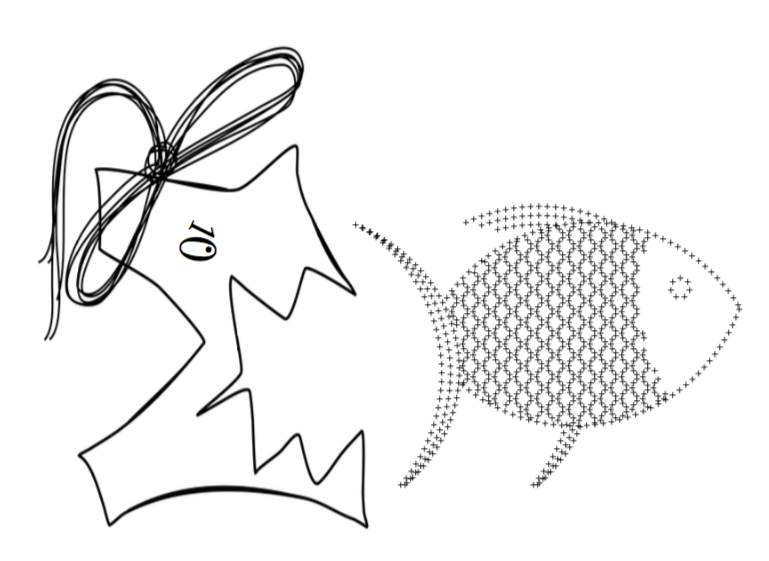
\includegraphics[height=10.5cm]{ExamplePoster/figs/outreachlogo.png}
\end{textblock}

\begin{textblock}{8}(4,1)
\titlepage
\end{textblock}

\begin{textblock}{7.25}(0.5,3.0)

%this needs help
\begin{block}{Introduction}
Over the last decade, McMaster Start Coding has taught over 15,000 students Computer Science and has created new frameworks and tools to help K-12 students learn.  In response to the COVID-19 pandemic, we developed and provided several virtual camps delivered for free to students through the summer using the Zoom platform and our online learning platform MacOutreach.Rocks.

\end{block}

\begin{block}{3D Object API}
An Elm-based application programming interface (API) was created to mimic the 2D 
\href{https://package.elm-lang.org/packages/MacCASOutreach/graphicsvg/latest/GraphicSVG}
{\texttt{GraphicSVG}} API our campers learned previously, allowing them to easily learn the API. Thus, 
we minimized the API learning curve and students instead focused on learning how to think three dimensionally. 

Some example functions and their type signatures:

\begin{itemize}
    \item \texttt{cube : Float -> Material coordinates -> Object coordinates} 
    \begin{itemize}
        \item An example of a "Mold" for creating 3D objects. 
        \item Only the size (Float) is given initially; it is then piped into another function to apply the material
    \end{itemize}
    \item \texttt{matte : Color -> Mold coordinates a -> Object coordinates} 
    \begin{itemize}
        \item One of our functions for applying a material to a \texttt{Mold}. We have many different molds, including the cube function above. This one applies a solid colour, non-reflective material.
        \item The colour for this function comes from the \texttt{elm-color} module, rather than \texttt{GraphicSVG}.
    \end{itemize}
    \item \texttt{move3D : Dimension -> Object coordinates -> Object coordinates } 
    \begin{itemize}
        \item One of our functions for transforming objects. Others include rotation and scaling.
        \item \texttt{Dimension} is a type alias for \texttt{(Float, Float, Float)}. For simplicity, all units are in centimetres.
    \end{itemize}
\end{itemize}

\end{block}

\begin{block}{3D Bee Simulator Game}
For the first 3D camp, campers were placed in groups to design a 3D bee pollination simulator. Campers
were tasked with designing both assets (including bees, flowers and hives) for the game and the layout of 
the level. The teams' levels were then combined into a large game at the end of the week.
Here are some examples of assets the campers made for the game:

\begin{figure}
    \centering
    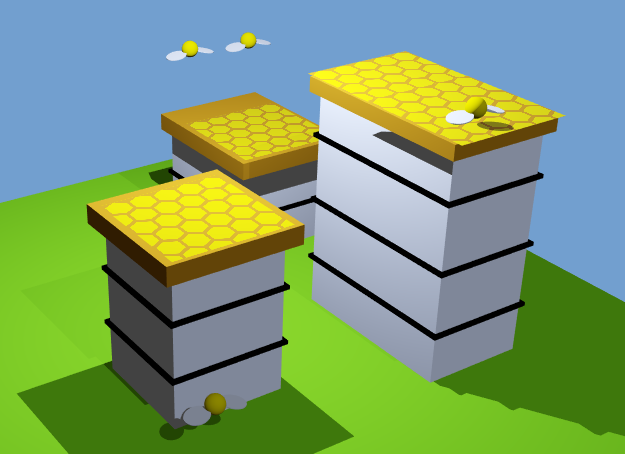
\includegraphics[height = 12 cm]{ExamplePoster/figs/BeeGamePictures/Beehives.PNG}\hspace{0.3cm}
    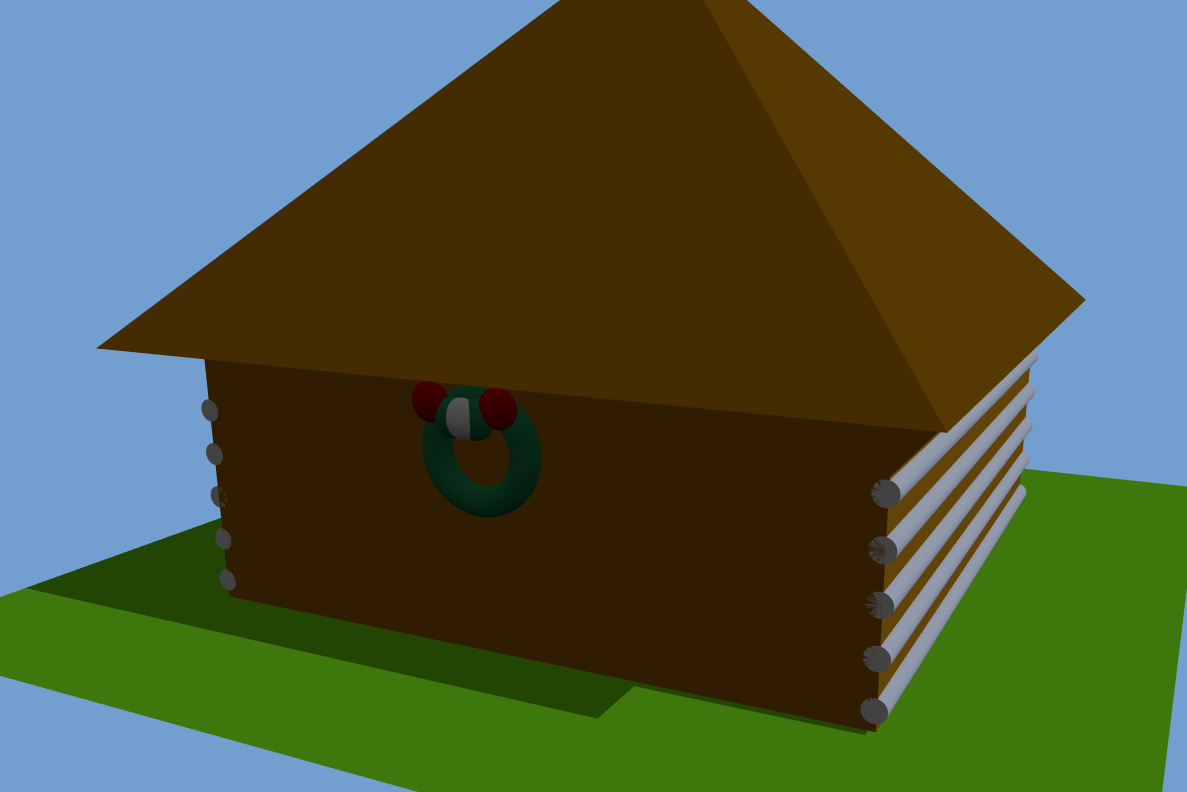
\includegraphics[height = 12 cm]{ExamplePoster/figs/BeeGamePictures/GingerbreadHouse.PNG}\\
    \vspace{0.5cm}
    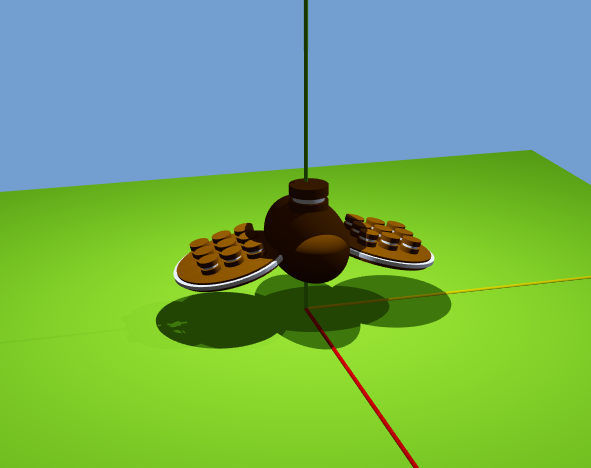
\includegraphics[height = 11 cm,trim={3.5cm 2.5cm 3cm 4cm},clip]{ExamplePoster/figs/BeeGamePictures/OreoBee.PNG}
    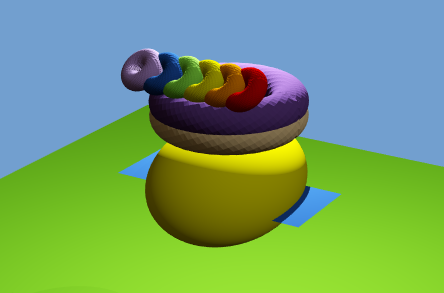
\includegraphics[height = 11 cm]{ExamplePoster/figs/BeeGamePictures/DoughnutBee.PNG}
    \caption{Assets created by middle school students in the camp (shared with permission). Top left: A set of beehives with bees flying around; top right: a gingerbread house; bottom left: a bee made out of cookies; bottom right: a bee made out of doughnuts. One of the teams in the camp decided to have a candy theme for their area in the game.}
\end{figure}

\end{block}

\begin{block}{Open Source Modules Used}
Several, fully open source modules were used in the creation of both activities:

\begin{itemize}
    \item \texttt{elm-3d-scene} provides an interface to WebGL graphics
    \item \texttt{elm-3d-camera} provides functions for working with virtual 3D cameras inside a 3D scene
    \item \texttt{elm-units} provides the ability to express and manipulate scientific units
    \item \texttt{elm-geometry} provides the ability to manipulate 3D and 2D geometric objects
    \item \texttt{elm-physics} allows the simulation of real-time 3D and 2D physics scenes with rigid bodies
\end{itemize}

\end{block}


\end{textblock}



\begin{textblock}{7.25}(8.25,3.0)

\begin{block}{3D Physics Slot}
The 3D Physics slot on our online code compilation system allows students to create 3D objects
and apply forces to them, simulating linear and angular acceleration and collisions. This was made
possible in large part by the \texttt{elm-3d-scene} and \texttt{elm-physics} packages.
\begin{figure}
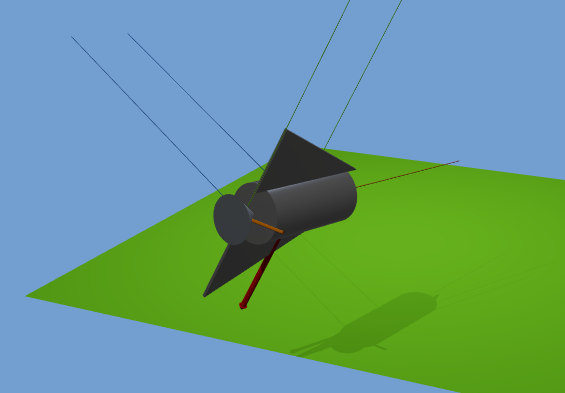
\includegraphics[height = 10 cm]{ExamplePoster/figs/BeeGamePictures/OldPlanePhysics.png}
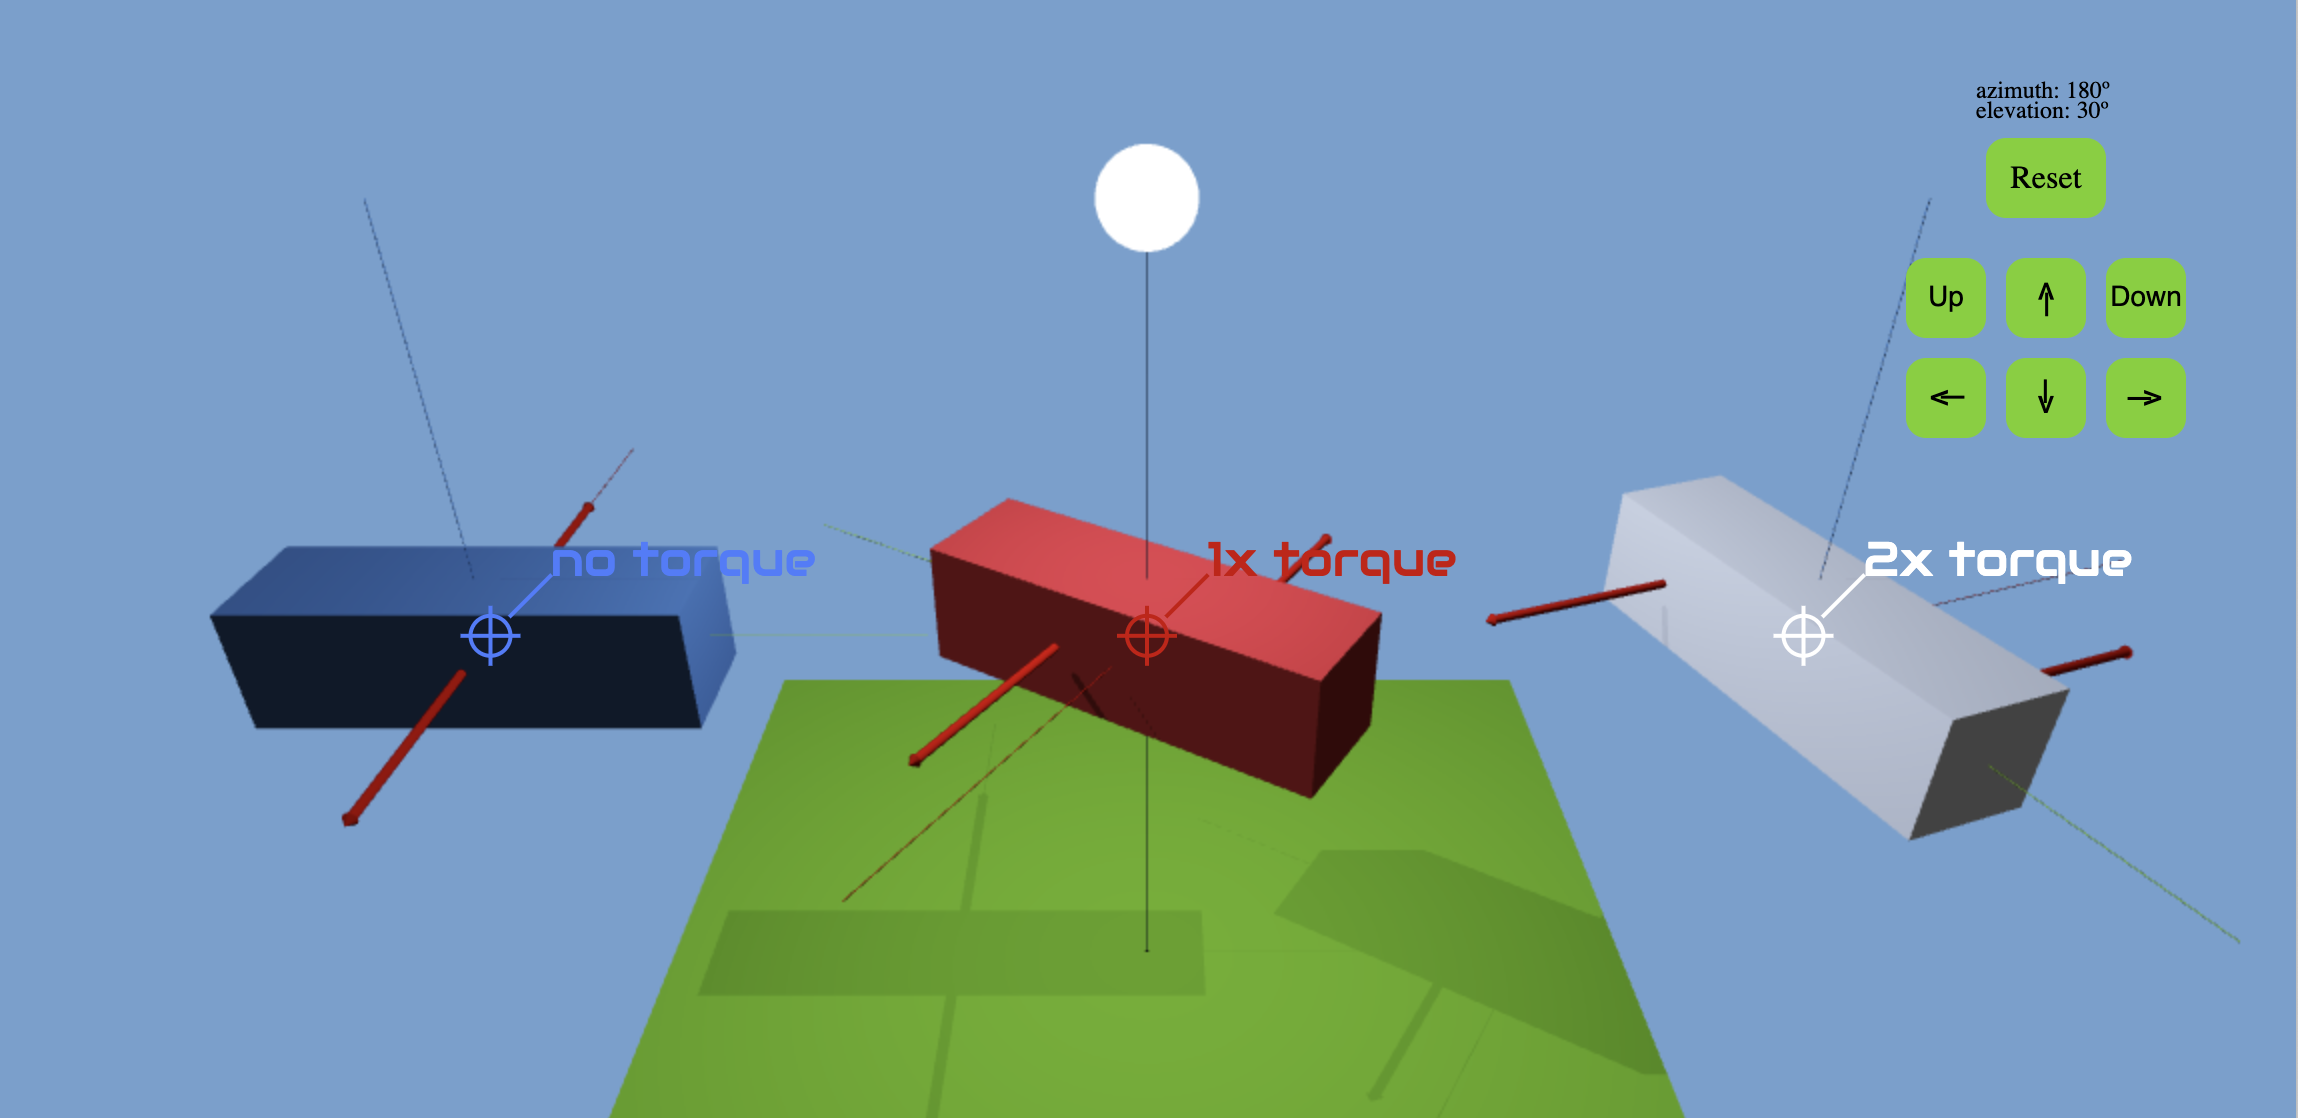
\includegraphics[height = 10 cm]{ExamplePoster/figs/PhysicsSlot.png}
\caption{In our Physics Slot, students are free to explore and get familiar with 3D forces and collisions. Students can visualize the forces (red arrows) and see a realtime simulation of movements. Left: visualizing forces on a rocket as an example. Right: An example of how placing forces further from the centre of gravity causes more torque and 
thus a higher angular acceleration.}
\end{figure}
\vspace{-5mm}
\end{block}

\begin{block}{3D Space Simulator Game}
To plan a more advanced 3D camp, students were surveyed about the type of game they would like to make
next. The idea of a space game was the highest-voted activity. Thus, our advanced 3D camp had campers
create and simulate 3D spaceships, complete with accurate simulated physics. A scene was set up to 
simulate flying from a space station to a satellite on a repair mission.
\end{block}

\begin{block}{Spaceship API}
To create a spaceship, students used skills acquired at the Bee Camp and special physics skills in the
spaceship camp. Using an Elm API, students specify the parts of their spaceship, including fuel tanks, 
boosters and angular velocity stabilizers. Then they can also program 
keyboard actions and autopilot routines to fly their spacecraft manually, semi-automatically or fully 
automatically.

\begin{figure}
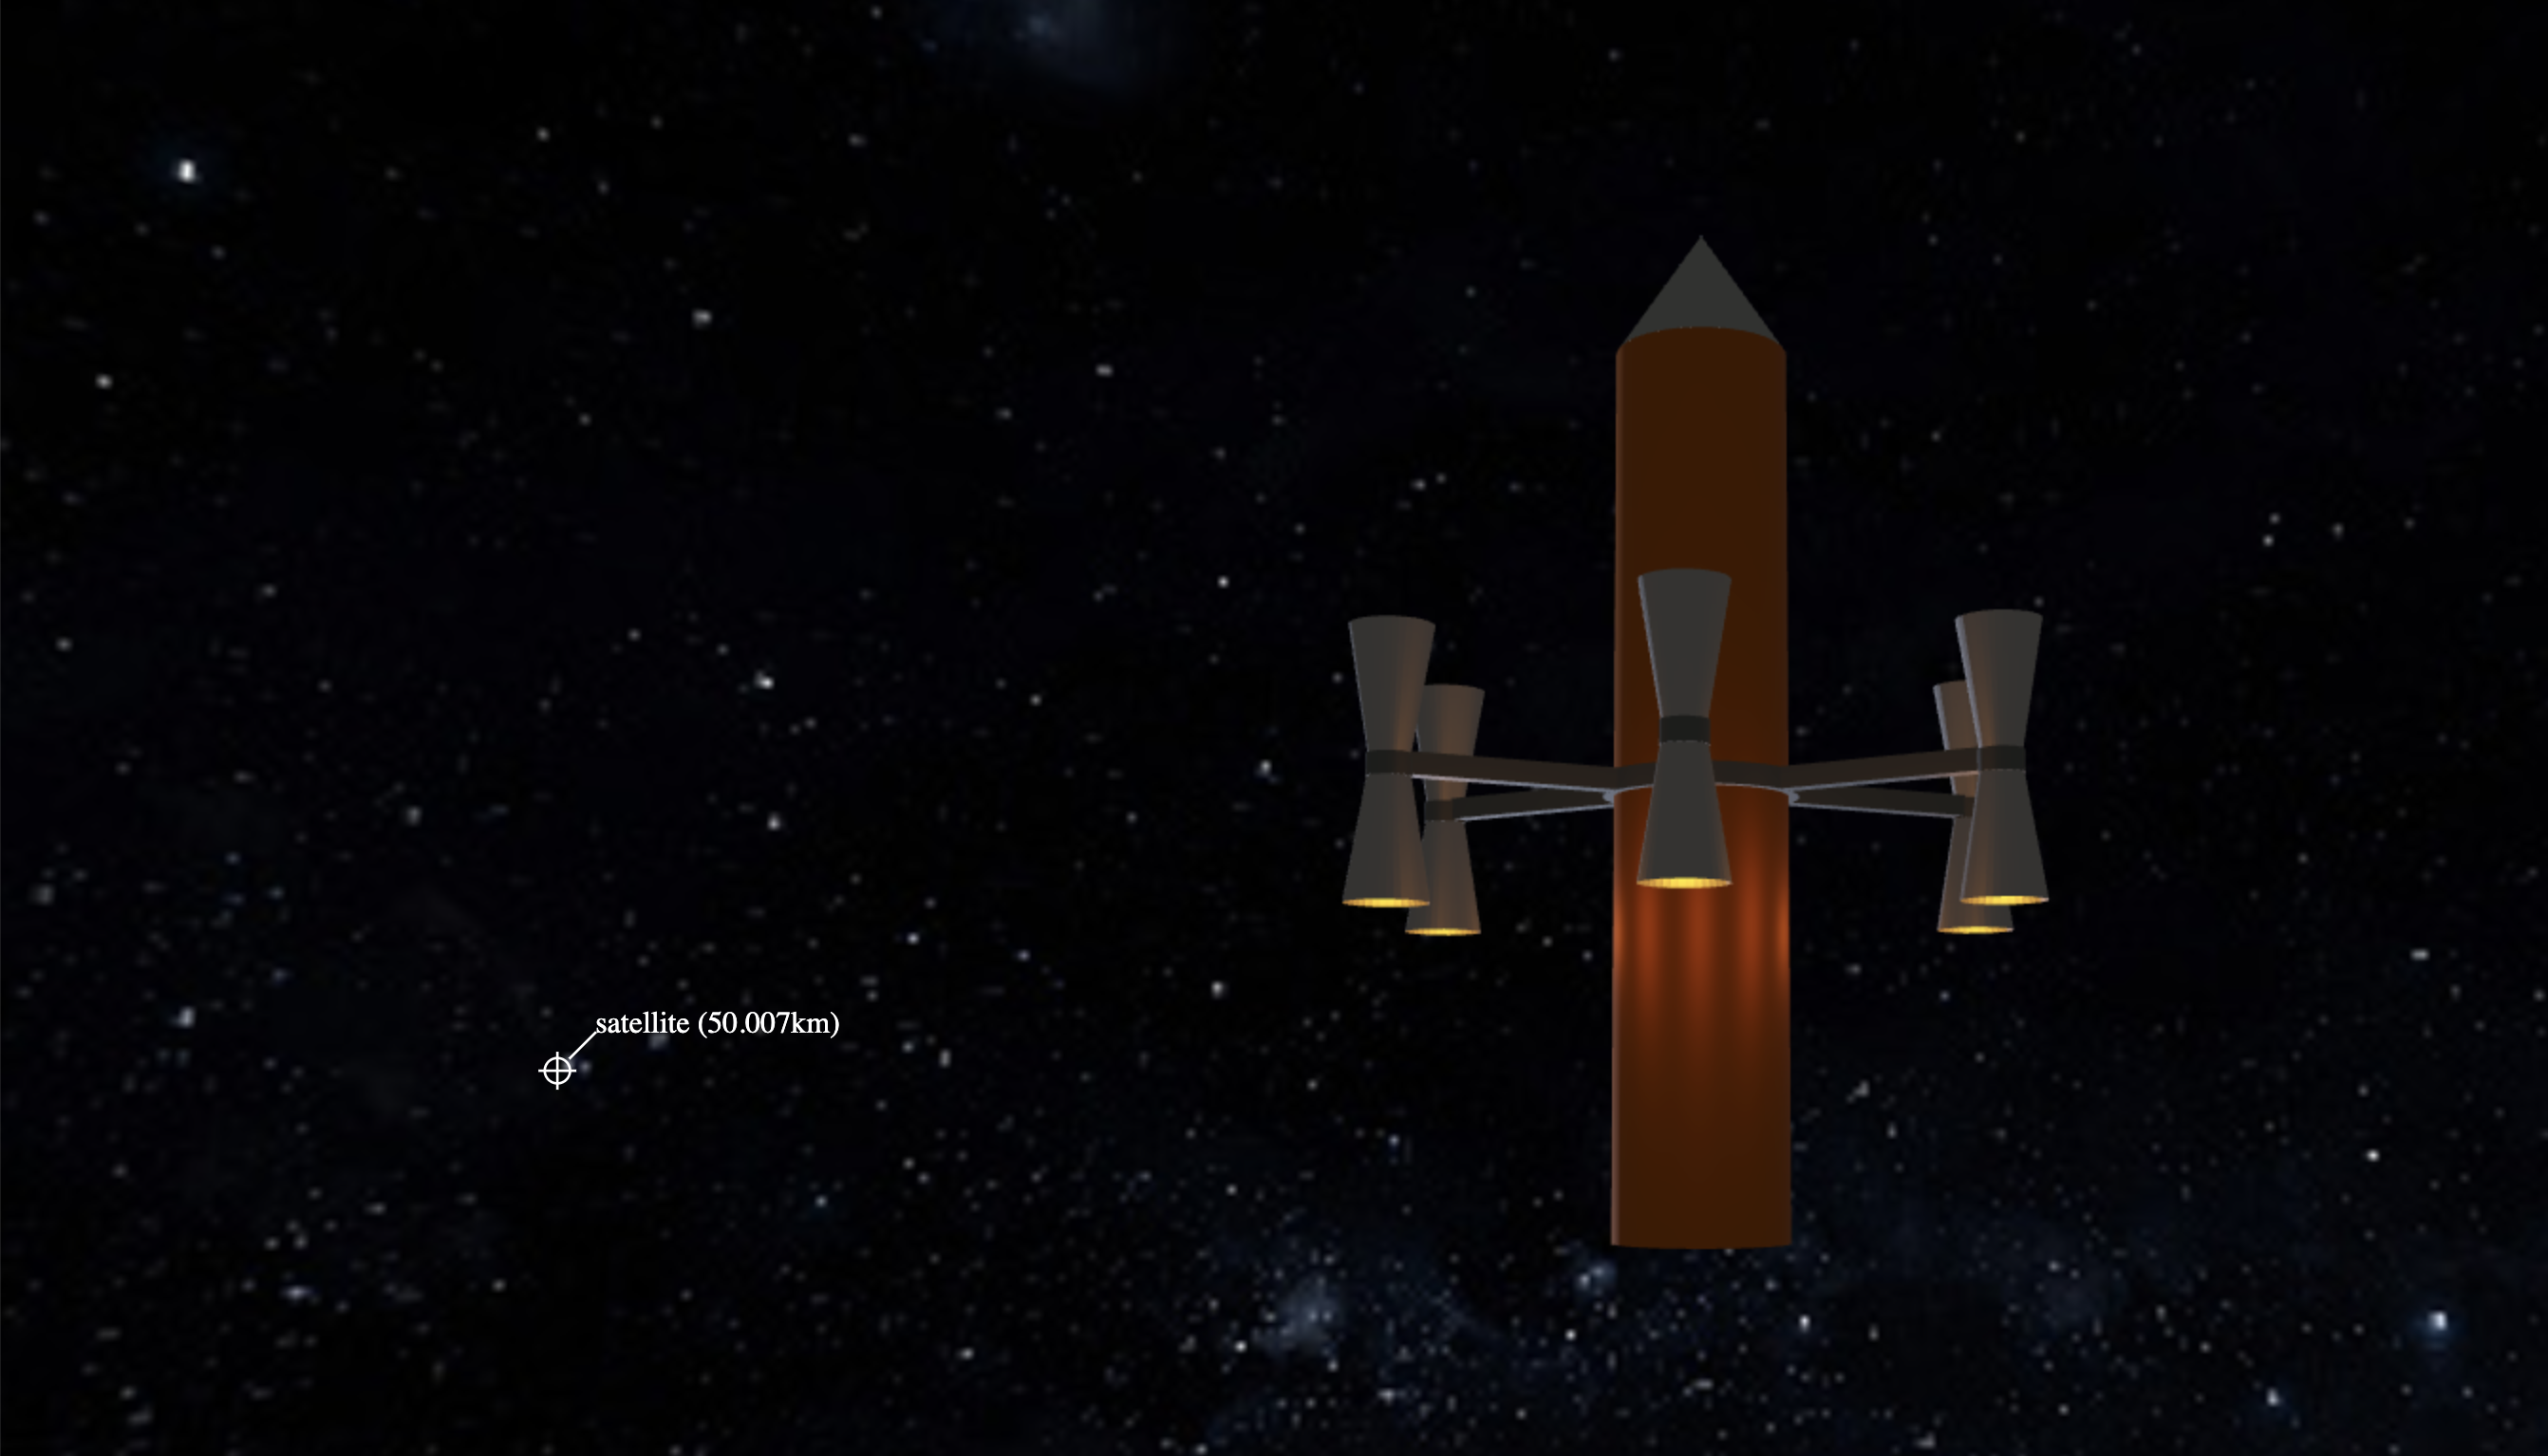
\includegraphics[height = 14cm]{ExamplePoster/figs/Rocket.png}
\caption{Students write code to design and build a rocket, which can then be flown manually or by
a student-specified autopilot program. They must iterate on their design to reach their goal and
optimize the amount of time it takes.}
\end{figure}
\end{block}

\begin{block}{Conclusions \& Future Work}
The 3D camps were anecdotally well-received by campers, who found the transition from 2D to 3D challenging
but manageable thanks to our familiar API. Future work includes testing students' knowledge of
general and rocket physics after completing the activities, as well as studies measuring students'
visualization skills after creating the 3D games. We would also like to open source the API.

\end{block}

\begin{block}{Thanks}
\footnotesize{\textit{Thanks to the McMaster Dean of Engineering and NSERC for funding. Thanks to all who gave help developing these tools, and to the many volunteers, co-op students and graduate students who helped make the camps a success. Special thanks to package author and Elm community member Ian 
Mackenzie for providing guidance and support while developing our tools using his libraries. Most of all, thanks to the campers for your endless passion, creativity and imagination.}}
\end{block}


\begin{figure}[htbp]
\centering

\includegraphics[height=5cm]{nserc-logo.jpg}
\hspace{1cm}

\includegraphics[height=5cm]{elm-logo.png}

\end{figure}
\end{textblock}




\end{frame}
\end{document}
